\section{System Architecture}
A custom Android application (Figure \ref{app}) was designed to be used during the study. This application collected and locally stored sensor data from a Microsoft Band smartwatch in a CSV file. The following data was collected from the Microsoft Band:
\begin{itemize}
	\item Accelerometer
	\item Gyroscope
	\item Pace
	\item Speed
	\item Distance traveled
	\item Motion type (idle, walking, etc.)
	\item Heart rate
	\item Pedometer
	\item Skin temperature
	\item Ultraviolet level
	\item Contact (if smartwatch is on)
	\item Calories burned
\end{itemize}
Additional data continuously collected and stored in the CSV by the application included:
\begin{itemize}
	\item GPS coordinates from the smartphone 
	\item Button that was pressed whenever the user took a drink
	\item Input field used to periodically record the BAC measured by a separate breathalyzer.
\end{itemize} 

\begin{figure}[H]
	\centering
	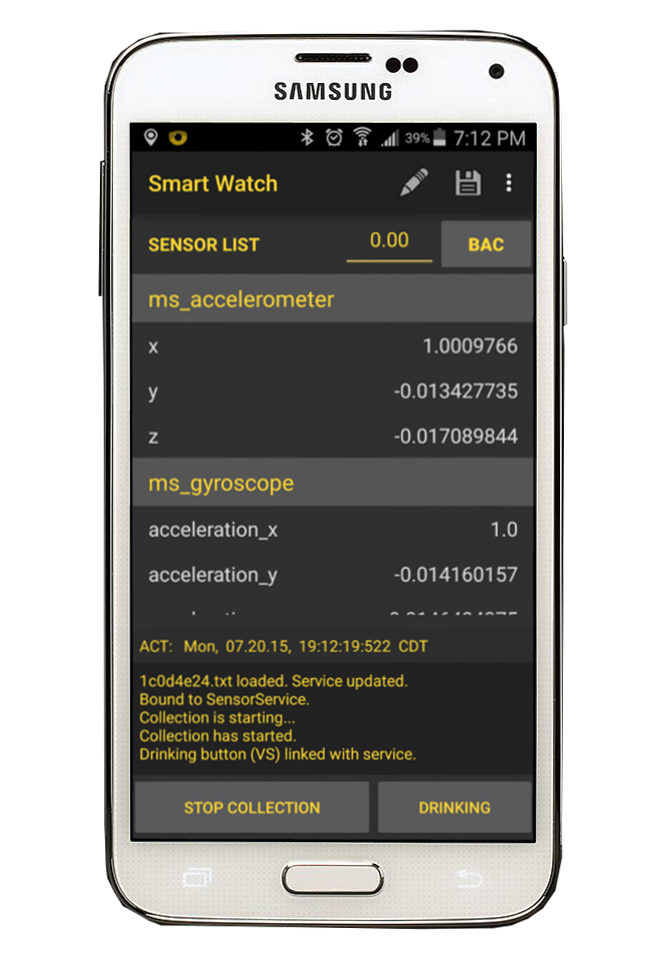
\includegraphics[scale=.20]{../figs/smartwatch.png}
	\caption{Capture of the Android application}
	\label{app}
\end{figure}

User information was also recorded and stored through the application before data collection began. Each user was given an unique user id (UUID) and the user profile included age, sex, body mass index, and blood type which was also stored locally as a JSON file.

After the data had been collected, the stored csv file and json file were uploaded to the web server and data inserted into mySQl database by a php script. Data stored on the MySQL database was then displayed on a web client by a geographical map. 

\begin{figure}[H]
	\centering
	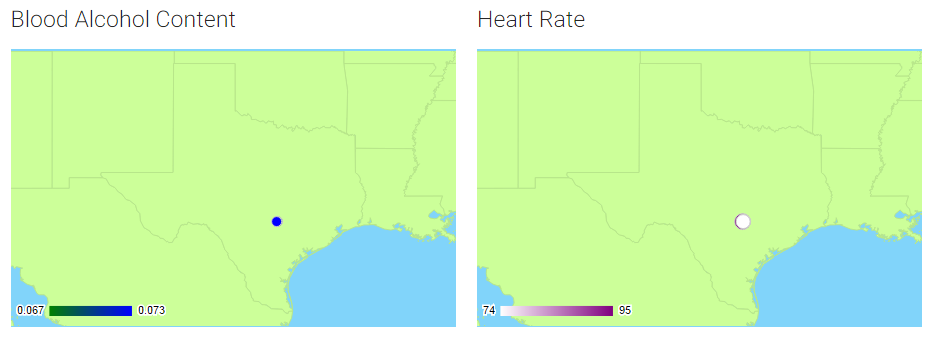
\includegraphics[scale=.35]{../figs/webpage.png}
	\caption{Current data visualization}
	\label{webpage}
\end{figure}

As of now, the web client displays the last sample for each user at the recorded location (Figure \ref{webpage}). Ideally in future systems, many samples will be averaged across regions (Figure \ref{concept}). 

\begin{figure}[H]
	\centering
	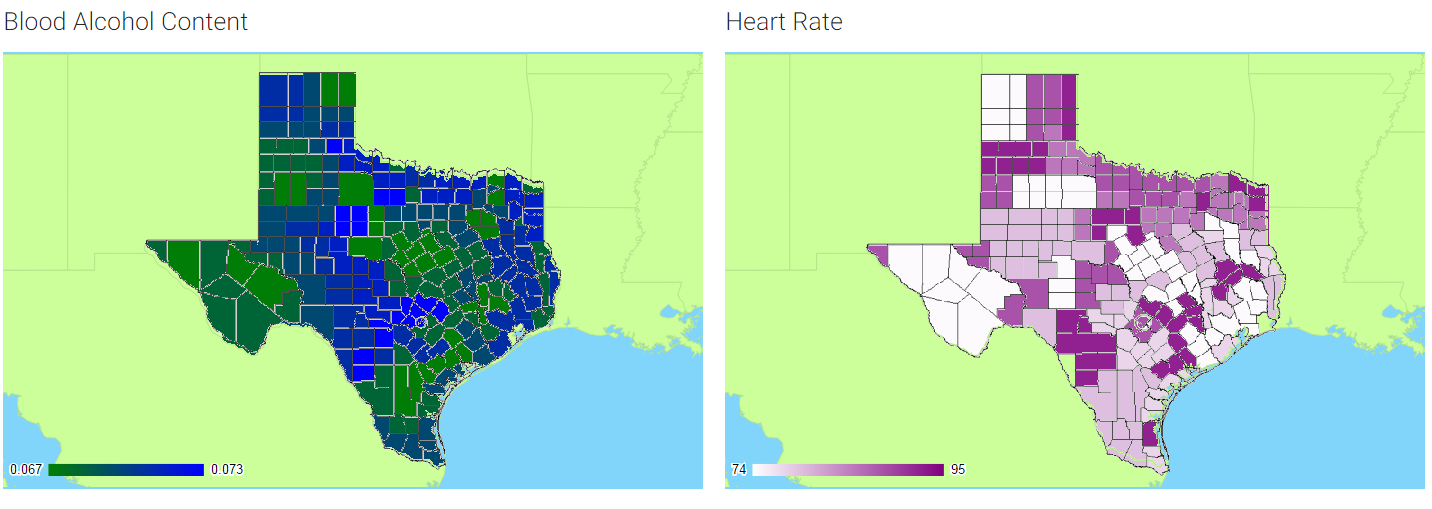
\includegraphics[scale=.23]{../figs/webconcept.png}
	\caption{Ideal data visualization}
	\label{concept}
\end{figure}

The collected data was also used to train a machine learning model which would be implemented in a future Android application to predict user BAC or drunkenness. 

\begin{figure}[H]
	\centering
	\includegraphics[scale=.30]{../figs/applicationsystem.png}
	\caption{Application system}
	\label{appsystem}
\end{figure}

Representation of this system can be found in Figure \ref{overallsystem}.

\begin{figure}[H]
	\centering
	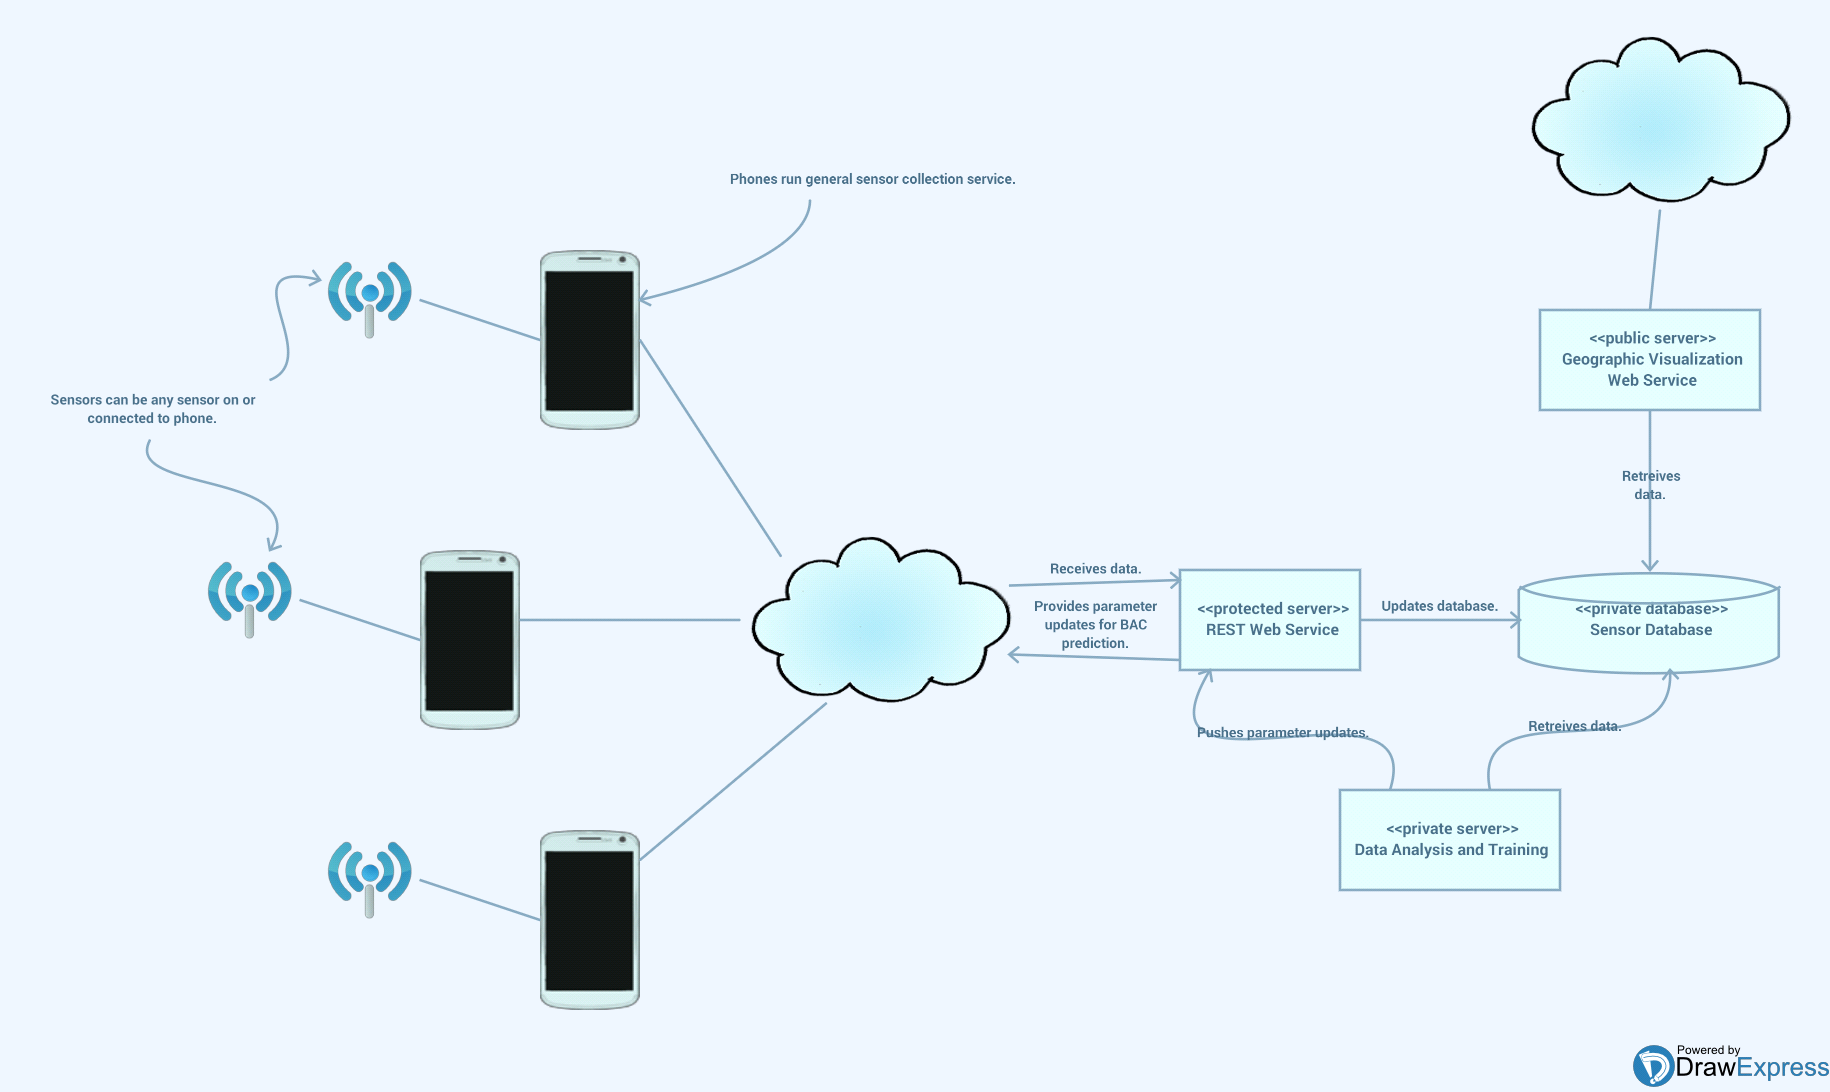
\includegraphics[scale=.14]{../figs/overall_system.png}
	\caption{Overall system}
	\label{overallsystem}
\end{figure}
